\section{Introduction}

La structure de ce document et certaines parties sont inspirées de
\cite{guide}.

L'objectif de ce guide est de donner un cadre à l'écriture de rapports 
de projet
à l'\gls{enstab}.
Il vient compléter le document d'aide à la
rédaction du rapport de stage opérateur \og{}Consignes pour la rédaction d'un
mémoire\fg{} disponible sur moodle à l'adresse 
\url{https://moodle.ensta-bretagne.fr/course/view.php?id=408} (section 4). 


La section \ref{sec:gen} présente les généralités sur la nature d'un rapport
de projet. La section \ref{sec:struct} décrit la structure attendue d'un rapport de
projet.
Puis, la section \ref{sec:regles} décrit les règles méthodologiques et
typographiques à respecter lors de la rédaction.
Enfin, la section
\ref{sec:outils} offre un aperçu des outils contribuant à l'écriture d'un rapport.


\section{Généralités}
\label{sec:gen}

En rédigeant un rapport, vous laissez une trace de votre travail, qui restera
disponible sur le long terme. Il faudra donc veiller à la qualité du fond
comme de la forme.

Afin d'être largement compris, le rapport doit privilégier une
écriture simple (mais non simpliste) faite de phrases courtes,
employant un vocabulaire explicite. Tous les acronymes doivent être explicités
et tous les termes techniques expliqués.

L'orthographe contribue à l'image que vous laissez de vous-même. Si les
correcteurs orthographiques sont d'un usage indispensable, ils ne remplacent
jamais une relecture soigneuse.
De plus, les usages typographiques de la langue employée doivent être respectés.

Avant l'entamer la rédaction d'un rapport, les réponses à quelques questions
fondamentales sur le rapport vous permettront de cadrer votre travail.

\subsection*{Pourquoi ?}

La réponse à cette question permet de définir la longueur du
document et son style, et bien entendu la nature du contenu.

\subsection*{Pour qui ?}

La réponse à cette question permet de définir la teneur des propos, les
notions que le lecteur maîtrise et celles qu'il faut détailler. Elle permet
également de cibler l'analyse à effectuer. Dans certains cas, elle permet
également de fixer le degré de confidentialité et
les modalités de diffusion.

\subsection*{Pour quand ?}

Cette réponse vous permet de gérer votre temps. Attention, l'écriture de
certaines parties nécessite un travail de recherche ou d'analyse préalable. De
plus, vous 
pouvez avoir à collecter des informations auprès de tiers dont vous ne
maîtrisez pas toujours les contraintes.

\subsection*{Pour combien de temps ?}

En répondant à cette question, vous allez définir la durée
d'utilisation du document~; vous en déduirez l'utilité d'en gérer des versions
consécutives.


\section{Structure du rapport}
\label{sec:struct}

Il n'y a pas de forme unique et universelle pour un rapport.
Néanmoins, la structure devra toujours comporter des éléments qui en
permettent l'utilisation efficace.\index{Structure (rapport)}
Dans tous les cas le rapport devra être paginé et le texte justifié.

 Le rapport devra \emph{obligatoirement} contenir~:
 \begin{itemize}
 \item un résumé~; 
 \item une page titre~;
 \item une table des matières~;
 \item une introduction~;
 \item un développement~; 
 \item une conclusion~;
\item une bibliographie.
 \end{itemize}

%et \emph{pratiquement systématiquement}~:
%\begin{itemize}
%\end{itemize}

\emph{Dans la plupart des cas}, on trouvera  également~:
\begin{itemize}
\item une liste de mots-clés~;  
\item une table des figures ou illustrations~;
\item des remerciements~;
\item une ou plusieurs annexes.
\end{itemize}

\emph{Dans certains cas}, il contiendra enfin~:
\begin{itemize}
\item un index~;
\item un glossaire.
\end{itemize}

Voyons les caractéristiques de ces différents éléments.

\subsection{Page de titre}

La page de titre doit permettre d'identifier le document. Pour cela, elle doit
comprendre~: \index{Page de garde}
\begin{itemize}
\item un titre~;
\item le type du document (par exemple \og{}Rapport de projet\fg{})~;
\item le nom du ou des auteurs du document~;
\item la date de parution (ou de remise du rapport) et éventuellement le
  numéro de version~;
\item le nom et le logo de l'organisme dont est issu l'auteur (par exemple
  \textsc{Ensta} Bretagne).
\end{itemize}

\subsection{Résumé}

Le résumé fait la synthèse du projet en une page au maximum. Il
devra contenir une brève description du problème et des objectifs du projet,
mentionner les résultats les plus
importants et dresser une conclusion. Dans le résumé il faut surtout mettre en
évidence les résultats car ce sont eux qui rendent mieux compte de votre
travail et donnent l'envie de lire votre rapport. 

Le résumé est souvent accompagné de quelques mots-clés et il est, dans
certains cas, traduit en une ou plusieurs langues.\index{Resume@Résumé}

\subsection{Table des matières}

Encore baptisée \og{} sommaire \fg{}, la table des matières permet de
synthétiser, en début de document, les différents chapitres qui y sont
traités. Elle doit faire
référence à la pagination du document pour permettre au lecteur
d'accéder directement à toute partie du document.\index{Table des
  matieres@Table des matières}\index{Sommaire} 

La table des matières se génère automatiquement ; ne la créez pas
manuellement, car vous pourriez oublier d'y apporter des
modifications.

\subsection{Introduction}

L'introduction doit permettre de situer le contexte de votre travail. En
particulier, elle doit~:\index{Introduction}
\begin{itemize}
\item présenter le contexte de l'étude~;
\item définir le problème que le projet cherche à résoudre, ainsi
    que le cadre dans lequel il s'inscrit~; 
\item définir le cadre du travail ; par exemple quelles ont été les
  contraintes, la méthodologie choisie~;
\item annoncer le plan, qui n'est pas un ennoncé plat des différentes parties,
  mais qui vise à définir l'orientation de la recherche, les hypothèses, le
  cheminement choisi pour tenter de répondre à la question.
\end{itemize}

%Il est également souhaitable de présenter les différentes parties et leur
%enchaînement.

\subsection{Développement}

Le développement est la partie substantielle de votre document. Il doit être
structuré et découpé en plusieurs parties. Les enchaînements entre les parties
doivent être fluides (par exemple grâce à une courte introduction en début de
partie et un court bilan à la fin). Il peut s'appuyer sur des compléments
d'information (notes de bas de page, références, annexes, glossaires ou listes
d'acronymes). N'hésitez pas à illustrer vos propos par des figures, tables
ou équations.

\subsubsection{Notes de bas de page}

Les notes de bas de page servent à apporter un complément d'information
non essentiel. Le texte doit pouvoir être compris sans y faire appel.
Elles sont très utiles lorsque l'on veut que le document puisse avoir
plusieurs niveaux de lecture.\index{Notes de bas de page}

\subsubsection{Figures et graphiques}

Si on se réfère à \cite{tufte}, les graphiques de qualité doivent
communiquer au lecteur un maximum d'information en un minimum de temps. Lors
de l'utilisation de figures, vous vous attacherez à respecter les règles
suivantes~:\index{Figures}
\begin{itemize}
\item Toutes les figures doivent posséder un titre et être citées dans le
  document (par exemple \og{}la figure \ref{fig:fract} nous montre que
  \ldots{}\fg{})~; la numérotation des figures doit être gérée
  automatiquement.
\item La mise en page doit être homogène à l'intérieur d'un graphique.
\item Des graphiques séparés servant de base à des comparaisons doivent avoir
  une mise en page cohérente. Ils doivent notamment être représentés à la même
  échelle et utiliser la même palette de couleurs.
\item Selon \cite{tufte}, pour de petits ensembles de
  données\footnote{moins de 20 données}, les 
  tableaux sont plus informatifs que les graphiques.
\item Les graphiques doivent être correctement étiquetés~:
  \begin{itemize}
  \item si $x$ représente les abscisses et $y$ les ordonnées, faites en sorte
    que $y=f(x)$ plutôt que $x=f(y)$~;
  \item n'oubliez pas les unités sur les axes, typiquement entre crochets
    (voir figure \ref{fig:fract}).
  \end{itemize}
\item Chaque graphique doit être analysé dans le corps du document.
\end{itemize}

\begin{figure}[htbp]
  \centering
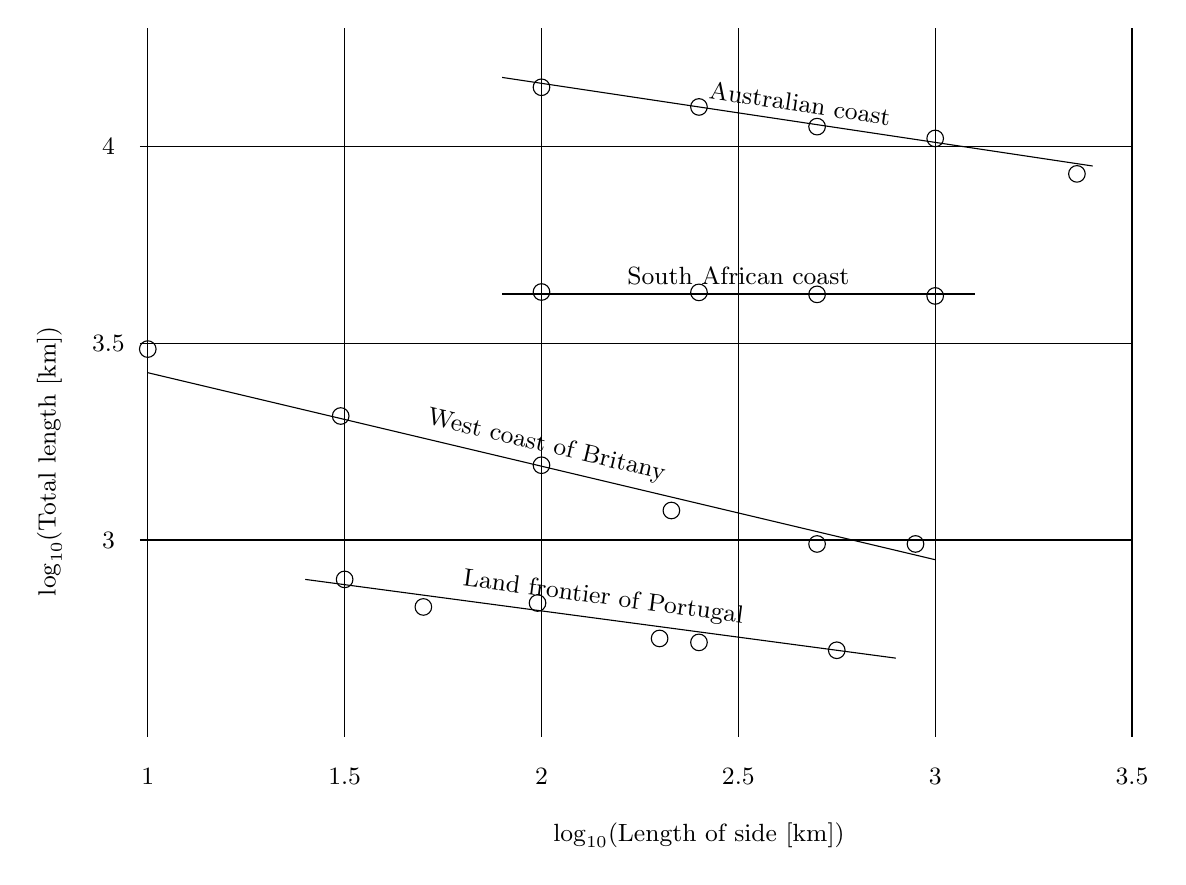
\begin{tikzpicture}[x=1cm,y=1cm,scale=5,font=\small]
  \draw[step=0.5] (0.98,2.5) grid (3.5,4.3);
  \foreach \x/\y in {1/3.485,1.49/3.315,2/3.19,2.33/3.075,2.7/2.99,2.95/2.99,1.5/2.9,1.7/2.83,1.99/2.84,2.3/2.75,2.4/2.74,2.75/2.72,2/3.63,2.4/3.629,2.7/3.624,3/3.62,2/4.15,2.4/4.1,2.7/4.05,3/4.02,3.36/3.93} {
    \draw (\x,\y) circle (0.6pt);
  }
  \draw (1,3.425) -- node[sloped, above] {West coast of Britany}
  (3,2.95);
  \draw (1.4,2.9)-- node[sloped, above] {Land frontier of Portugal} (2.9,2.7);
  \draw (1.9,3.625)-- node[sloped, above] {South African coast} (3.1,3.625);
  \draw (1.9,4.175)-- node[sloped, above] {Australian coast} (3.4,3.95);
  \foreach \x in {1,1.5,...,3.5} {
    \draw (\x,2.4) node {\x};
  }
  \node at (2.4,2.25) {$\log_{10}$(Length of side [km])};
  \foreach \y in {3,3.5,4} {
    \draw (0.9,\y) node {\y};
  }
  \node[rotate=90] at (0.75,3.2) {$\log_{10}$(Total length [km])};
\end{tikzpicture}
  \caption{Dimension fractale de traits de côte de différents pays ; relation entre longueur et pas}
  \label{fig:fract}
\end{figure}

De manière générale, prenez garde à la lisibilité de vos figures. Pensez
également que la lisibilité est différente sur écran, sur une impression
couleur, ou sur une impression en noir et blanc.

Concernant le format des figures, préférez dans la mesure du possible les
formats vectoriels\footnote{qui ne se dégradent pas lors des changements de
  taille} comme \emph{eps}, \emph{pdf} ou \emph{svg}. Si vous optez pour un
format image sachez que, de part son algorithme de compression, le format
\emph{jpg} dégradera fortement le texte~; préférez-lui le format \emph{png}.

Dans le cas où la figure est issue d'une capture d'écran, pensez à ajouter un
habillage et gardez toujours à l'esprit la lisibilité de la figure~; si
nécessaire, modifiez les couleurs dans un outil de traitement
d'images\footnote{Par exemple \textsc{gimp}}. 

\subsubsection{Tables}

De la même manière que les figures, les tables servent à illustrer certains
éléments du rapport. Elles doivent posséder un titre et être
référencées dans le corps du document. Il faut prendre garde à leur
lisibilité. Un exemple \emph{à ne pas suivre} est présenté table
\ref{tab:tab1} (table extraite du manuel de \LaTeX). Dans cet exemple, les
lignes (horizontales et verticales) sont 
trop nombreuses et nuisent à la lisibilité, les alignements sont erratiques,
les unités ne sont pas correctement indiquées et les nombres sont représentés
avec des précisions différentes. Enfin, les titres de chaque colonne ne sont
pas apparents.\index{Tables}

\begin{table}[htbp]
  \centering
\begin{tabular}{||l|lr||} 
\hline
\hline
~~~~~gnats     & gram      & 013.65\euro \\ \cline{2-3}
          & each      & .01 \\ \hline
gnu       & stuffed   & 92.5 \\ \cline{1-1} \cline{3-3}
~~~emu       &           & 33.33 \\ \hline
armadillo & frozen    & 8.9887 \\ \hline
\end{tabular}
  \caption{Une table très mal présentée}
  \label{tab:tab1}
\end{table}

La table \ref{tab:tab2} corrige tous les problèmes de la table
\ref{tab:tab1}. Cette fois, la table est lisible et elle peut apporter un
complément d'information au texte.

\begin{table}[htbp]
  \centering
\begin{tabular}{@{}llr@{}} 
  \toprule
  \multicolumn{2}{c}{\textbf{Item}} \\ 
  \cmidrule(r){1-2}
  \textbf{Animal} & \textbf{Description} & \textbf{Price (\euro)}\\ 
  \midrule
  Gnat  & per gram  & 13.65 \\
           & each      & 0.01 \\
      Gnu   & stuffed   & 92.50 \\
      Emu   & stuffed   & 33.33 \\
      Armadillo & frozen & 8.99 \\ 
      \bottomrule
\end{tabular}
  \caption{Une table correctement présentée}
  \label{tab:tab2}
\end{table}

\subsubsection{Équations}

Il est parfois plus simple de décrire un processus par des équations que par
du texte. 
De la même manière que les figures et les tables, les équations
doivent être numérotées, et être référencées dans le texte du
rapport. \index{Equations@Équations}

Exemple~: Soit $S={p_1,\ldots,p_n}$ un ensemble fini de points de
$\nbR^d$. L'équation \eqref{eq:1} décrit l'enveloppe convexe de $S$.

\begin{equation}
  \label{eq:1}
  \mathcal C(S)=
  \left\{
    \sum_{i=1}^n\alpha_i p_i \mbox{ avec } \forall i, \alpha_i\geqslant 0
    \mbox{ et } \sum_{i=1}^n\alpha_i =  1
  \right\}
\end{equation}

\subsection{Conclusion}

La conclusion est une sythèse de votre travail et doit en faire un bilan
(critique) vis-à-vis des 
objectifs initiaux. 
Vous devez ici mentionner vos doutes et certitudes quant à
vos résultats~; n'hésitez-pas à fournir des pistes pour un travail à venir ou
des explications pour un travail non abouti.

\index{Conclusion}

\emph{Introduction et conclusion sont des parties essentielles d'un
  document. En les lisant, le lecteur doit pouvoir se faire une idée
  précise du contenu développé dans le corps du texte. Il est
  important d'y apporter le plus grand soin.}

\subsection{Bibliographie}

\paragraph{Remarque~:} ce document ne décrit pas la méthode
permettant de rechercher des références bibliographiques. Pour cela,
reportez vous à l'UV 1.4 \og{}Bibliographie\fg{} accessible sur moodle~:
\url{https://moodle.ensta-bretagne.fr/course/view.php?id=617}.

La bibliographie reprend toutes les références qui ont servi de support lors de
votre travail. Elle ne doit contenir que les références lues et qui sont
citées dans le corps du document.\index{Bibliographie}

Afin de faciliter la maintenance et l'homogénéité de la bibliographie, il est
conseillé de s'appuyer sur un outil de gestion de références tel que
\emph{Zotero} ou BibTeX. Certains outils\footnote{\emph{Zotero} par exemple,
  mais également des sites tels que \url{https://www.diigo.com} ou
  \url{http://www.citethisforme.com}}
permettent une gestion collaborative des références.

Exemple~: \emph{Selon \cite{tufte}, pour de petits ensembles de
  données, les tableaux sont plus informatifs que les graphiques.}

L'utilisation de références bibliographiques permet~:
\begin{itemize}
\item d'indiquer les résultats et conclusions qui viennent d'autres
  travaux (ne pas citer ses sources constitue une faute grave)~;
\item de donner plus de force à vos propos en vous appuyant sur des résultats
  reconnus par la communauté scientifique~;
\item de vous affranchir de l'écriture d'une démonstration ou d'un calcul~;
\item de citer les documents techniques sur lesquels vous vous appuyez~;
\item de donner des pistes d'exploration pour ceux qui veulent creuser
  certains points.
\end{itemize}

Il existe plusieurs styles classiques de bibliographie, comme par exemple le
format numéroté dans lequel les références sont indexées par un numéro entre
crochets. Les références sont alors ordonnées selon l'ordre d'apparition dans
le document.

\paragraph{Exemple de bibliographie numérotée~:}
\begingroup
\renewcommand{\section}[2]{}%
\begin{thebibliography}{1}
\bibitem{n1} Rudolf \textsc{Bayer} et Edward Meyers \textsc{McCreight}. ``Organization and
  maintenance of large ordered indexes''. In : \emph{Acta Informatica} 1.3
  (1972), p. 173--189.
\bibitem{n3} Benoît \textsc{Mandelbrot}. ``How long is the coast of Britain ?
  Statistical selfsimilarity and fractional dimension''. In: \emph{Science}
  156.3775 (5 mai 1967), p. 636.
\bibitem{n2} Kenneth Lee \textsc{Clarkson} et al. ``Approximating center points with
  iterated Radon points''. In : \emph{International Journal of
    Computational Geometry \& Applications} 06.03 (sept. 1996), p. 357--377.
\end{thebibliography}
\endgroup

~\\
Un autre format classique est le format alphabétique dans lequel les
références apparaissent dans l'ordre alphabétique et sont composées de lettres
suivies de deux chiffres représentant l'année. Ces lettres sont~:
\begin{itemize}
\item les trois première lettres du nom de l'auteur (s'il est seul)~;
\item les initiales des auteurs (s'ils sont deux ou trois)~;
\item les trois première lettres du nom du premier auteur suivies du symbole
  \og{}+\fg{} (s'il y a plus de 3 auteurs).
\end{itemize}

\paragraph{Exemple de bibliographie alphabétique~:}
\begingroup
\renewcommand{\section}[2]{}%
\begin{thebibliography}{WWW99}
\bibitem[BM72]{a1} Rudolf \textsc{Bayer} et Edward Meyers \textsc{McCreight}. ``Organization and
  maintenance of large ordered indexes''. In : \emph{Acta Informatica} 1.3
  (1972), p. 173--189.
\bibitem[Cla+99]{a2} Kenneth Lee \textsc{Clarkson} et al. ``Approximating center points with
  iterated Radon points''. In : \emph{International Journal of
    Computational Geometry \& Applications} 06.03 (sept. 1996), p. 357--377.
\bibitem[Man67]{a3} Benoît \textsc{Mandelbrot}. ``How long is the coast of Britain ?
  Statistical selfsimilarity and fractional dimension''. In: \emph{Science}
  156.3775 (5 mai 1967), p. 636.
\end{thebibliography}
\endgroup

\subsection{Annexes}

Les annexes regroupent les informations qui ne sont pas essentielles à la
compréhension générale du rapport et dont la présence dans le texte principal
nuirait à la fluidité de la lecture. Les annexes peuvent par exemple
contenir~:\index{Annexes}
\begin{itemize}
\item des démonstrations ou des calculs détaillés~;
\item des données techniques (de matériel par exemple)~;
\item des données brutes\footnote{uniquement si leur lecture apporte un
    complément d'information utile au lecteur.}~;
\item des glossaires et index.
\end{itemize}

\paragraph{Remarque~:} les programmes offrent rarement un intérêt dans les
annexes papier. Par contre, il peut être intéressant de les joindre sous forme
numérique\footnote{Par exemple dans un fichier archive \emph{7z}, \emph{tgz},
  \emph{tbz}, \emph{zip} ou \emph{rar}.}.

\subsection{Index et glossaire}

L'index et le glossaire sont placés dans les dernières pages du
document. L'index permet de retrouver les termes clés du document par une
recherche alphabétique~; il accélère la recherche d'information dans les
rapports volumineux.\index{Index}

Le glossaire permet de regrouper la description de termes techniques et de
sigles à la fin du document. Il permet une meilleure compréhension des
concepts dont l'explication n'est pas reprise en détail dans le texte.\index{Glossaire}

\section{Règles}
\label{sec:regles}

\subsection{Règles méthodologiques}

Le document doit être considéré comme un tout homogène et non comme
une compilation d'éléments disparates. Les auteurs sont solidairement
responsables (en contenu et en délai) de la totalité du document et
non uniquement de leur propre contribution.\index{Methodologie@Méthodologie}

La cohérence doit être recherchée à tous les niveaux afin de limiter
les ambiguïtés et d'améliorer la qualité du document produit. Avant la remise
d'un rapport conséquent, plusieurs phases de relecture sont généralement
nécessaires. Il est donc conseillé de commencer l'écriture du rapport dès que
possible. 

On veillera tout particulièrement à~:
\begin{itemize}
\item respecter la cohérence du style, des  temps et des modes employés ;
\item conserver le même mode de locuteur dans tout le texte (p.~ex.
  je, nous, l'équipe) ;
\item utiliser le même niveau de vocabulaire tout au long du texte. 
\end{itemize}

\subsection{Règles de typographie}

Les usages de typographie diffèrent d'une langue à l'autre. Si le rapport est
écrit en anglais, vous devez alors respecter les usages
anglo--américains~; consultez par exemple \cite{typoUS} pour des
informations détaillées. \index{Typographie}

De même, dans tous les cas où vous écrivez votre rapport en
français, il est important de respecter les règles de typographie française.
Dans ce cas,
la lecture de \cite{andreTypo} vous donnera un très bon aperçu des règles
à respecter et des écueils à éviter.

\subsection{Règles de présentation de résultats numériques}

Sauf dans le cas de valeurs dimensionnelles, les unités des résultats
numériques doivent toujours être précisées. 

Il est également important d'être conscient du sens implicite donné lors de la
présentation de valeurs numériques. En particulier, le nombre de chiffres
significatifs présenté traduit la fidélité de la mesure. Les chiffres
significatifs excessifs doivent être supprimés par arrondi.

\section{Outils d'aide à la production de documents}
\label{sec:outils}

Lors de votre scolarité à l'\gls{enstab}, vous avez généralement le
choix des outils utilisés pour la production de documents. 

\subsection{Traitement de texte et formateur de texte}

Un traitement de texte est un outil de mise en page de documents. Il est
généralement de type \gls{wysiwyg}\footnote{What You See Is What You Get}
et permet donc de voir l'aspect du document se modifier en continu. Dans cette
catégorie, les outils les plus connus sont \emph{Microsoft Word} et
\emph{LibreOffice}. Le formatage du texte est
obtenu par application de {\em styles}. Malheureusement, de nombreux
utilisateurs, insuffisamment formés, n'utilisent pas ou utilisent mal
cette fonctionnalité.

Le formateur de texte le plus connu est \LaTeX. Il procède en séparant le fond
et la forme du document et possède des bibliothèques de style qui permettent
de respecter les règles typographiques. Cet outil est généralement
non-\gls{wysiwyg} et requiert un certain investissement avant d'être
utilisé efficacement.

\subsection{Format des données}

La question du format de données se pose obligatoirement lors de la
manipulation de documents numériques. Le choix du format est souvent lié à
l'outil utilisé. Dans la mesure du possible, il est conseillé d'utiliser des
formats ouverts (c'est-à-dire dont la spécification est disponible).
Cette question est particulièrement importante lors du partage de document.

Voici quelques conseils pour vous aider dans le choix du format de données~:
\begin{itemize}
\item lors de la remise de documents \emph{non modifiables}, destinés à des
  sorties papier, il est conseillé d'utiliser le format \emph{pdf}~; soyez
  vigilants à l'intégration des polices de caractères lors de la génération et
  vérifiez systématiquement le résultat~; 
\item pour des documents consultables en ligne, le format \textsc{Html}
  conviendra parfaitement~;
\item pour l'échange de documents à modifier, les formats \emph{odt},
  \emph{rtf} et \emph{tex} sont ouverts~;
\item en ce qui concerne le format \emph{docx}, les spécifications existent,
  mais ne sont pas exactement respectées par \emph{Microsoft Word}, ce qui
  entraîne des problèmes de mise en page lors du passage par
  \emph{LibreOffice}\ldots{} Dans ce cas, il faudra veiller à ce que tous les
  rédacteurs utilisent la même version de \emph{Microsoft Word} ou de
  \emph{LibreOffice}. 
\end{itemize}

\subsection{Outils collaboratifs}

Rédiger un rapport à plusieurs est toujours une opération
délicate. L'utilisation d'outils collaboratifs permet de simplifier cette
phase, de manipuler plusieurs versions du document et de gérer les conflits.
Plusieurs solutions sont disponibles~:
\begin{itemize}
\item utiliser le mode \og{}Modifications\fg{} de \emph{Microsoft Word} ou de
  \emph{LibreOffice}~; l'échange de fichiers et la gestion de version doivent
  alors être assurés manuellement~;
\item utiliser un gestionnaire de version\footnote{Par exemple du \textsc{cvs}
  ou du \emph{subversion} hébergé sur le serveur
  \url{https://gforge.ensta-bretagne.fr/gf} ou une gestion décentralisée avec
  \url{https://github.com}.} pour héberger le code source
\LaTeX\footnote{Cette méthode ne fonctionne que si le document est au format
  texte.}~;
\item héberger le rapport sur un service \emph{cloud} tel que
  \emph{Google drive} ou \emph{Microsoft Office 365}.
\end{itemize}

\section{Conclusion}

Dans ce guide, les objectifs d'un rapport de projet ont
été précisés ainsi que la structure classique de son plan. Ensuite,
les règles de base pour sa rédaction ont été présentées, suivies d'un
rapide traitement des problématiques liées aux outils de production de
documents. 



%%% Local Variables: 
%%% mode: latex
%%% TeX-master: "../guide"
%%% End: 
